
This chapter investigates how maps between Boolean networks can respect both their dynamics and the dependencies recorded by their wiring diagrams. Conjugate Boolean networks have isomorphic phase spaces, yet their wiring diagrams need not be isomorphic: an arbitrary relabeling of states need not preserve changes in a single coordinate. We therefore begin with conjugacies that preserve the Hamming distance on the Boolean cube. These isometric conjugacies induce isomorphisms of wiring diagrams and provide a natural notion of isomorphism for Boolean networks. We show that every isometry is a composition of a coordinate permutation and coordinate complementations. Such maps form the group of signed permutations, or the Weyl group of type $B_n$, isomorphic to the wreath product $C_2\wr S_n$, where $S_n$ is the symmetric group.

Our main goal is to extend this connection between dynamics and wiring diagrams to reductions that aggregate several nodes into one. A semiconjugacy is a surjective state map $h$ satisfying $h\circ f=g\circ h$, so that the reduced network $g$ describes the evolution of the observed states. Requiring $h$ to be a contraction ensures that aggregation does not increase Hamming distances, but this alone does not ensure a corresponding relationship between wiring diagrams. We introduce a compatible node map $\phi$, which partitions the source nodes into blocks and requires each coordinate of $h$ to depend only on its assigned block. The main result, the edge-lifting theorem (Theorem~\ref{thm:compatible-edge-lifting}), shows that under these conditions every edge $a\to b$ in the reduced network lifts to an edge $i\to j$ in the original network with $\phi(i)=a$ and $\phi(j)=b$. Thus every dependency observed after reduction has a witness among the original dependencies. Examples show why compatibility is needed and how aggregation can erase source dependencies. The theorem gives a precise structural guarantee for network reduction and extends the preservation of wiring diagrams under isometric conjugacy to maps that identify states and group nodes.

\section{Conjugacy and isometric conjugacy}

\begin{definition}
    Let $f,g \colon \F^n\to \F^n$ be Boolean networks. A conjugacy from $f$ to $g$ is a bijection $h\colon \F^n\to \F^n$ such that $h\circ f=g\circ h$. When such a map exists, we say that $f$ and $g$ are conjugate and write $f\sim g$.
\end{definition}

We can represent the previous identity as the following commutative diagram.

\[
		\begin{tikzpicture}[scale=1.25, every node/.style={midway}]
			\matrix[column sep={4em,between origins}, row sep={2em}] at (0,0) {
				\node(A) {$\F^n$}; && \node(A1) {$\F^n$};\\
				\\
				\node(B) {$\F^n$}; && \node(B1) {$\F^n$};\\
			};
			\draw[->] (A) -- node(A2) [above] {$h$} (A1);
			\draw[->] (A) -- (B) node[anchor=east] {$f$};
			\draw[->] (B) -- (B1) node[anchor=south] {$h$};
			\draw[->] (A1) -- (B1) node[anchor=west] {$g$};
		\end{tikzpicture}
\]

Consequently, one may either (i) update a state via $f$ and subsequently relabel it through $h$, or (ii) first apply the relabeling $h$ and then update via $g$; in both cases the resulting state is identical. Furthermore, given a Boolean network $f$ and a bijection $h$, there exists a unique map $g$ that renders the corresponding diagram commutative, namely
\[
g = h\circ f\circ h^{-1}.
\]

Observe that the identity map conjugates $f$ to itself. If $h\circ f = g\circ h$, then composing on the right with $h^{-1}$ yields $f\circ h^{-1} = h^{-1}\circ g$, and hence $h^{-1}$ conjugates $g$ to $f$. Finally, if $h\circ f = g\circ h$ and $k\circ g = l\circ k$, then
\[
(k\circ h)\circ f \;=\; k\circ(g\circ h)\;=\; l\circ(k\circ h),
\]
which shows that $k\circ h$ conjugates $f$ to $l$. Therefore,
\begin{proposition}
    Conjugacy is an equivalence relation on Boolean networks.
\end{proposition}

\begin{example}\label{ex:and-or-conjugacy}
A paradigmatic instance of a structural correspondence is provided by the equivalence between OR-networks and AND-networks. Specifically, consider the maps $f,g\colon \F^3\to\F^3$ defined by
\[
f(x_1,x_2,x_3)= (x_1x_2x_3,\ x_1x_2,\ x_1x_3); \quad
g(y_1,y_2,y_3)= (y_1\vee y_2\vee y_3,\ y_1\vee y_2,\ y_1\vee y_3).
\]
The wiring diagrams associated with these two networks coincide; they are given below, where self-loops are understood and each edge is regarded as bidirectional:
\[
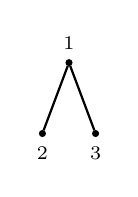
\begin{tikzpicture}[scale=.9,xscale=.75,every label/.append style={font=\scriptsize}]
 \tikzstyle{v} = [circle, draw, fill=black,inner sep=0pt, minimum size=.75mm]
    \tikzstyle{e} = [thick] 
    %%
    
        \node[v,label=above:{$1$}] (r) at (0,1) {};
        \node[v,label=below:{$2$}] (v1) at (-.5,0) {};
        \node[v,label=below:{$3$}] (v2) at (.5,0) {};
        \draw[e] (r)--(v1); \draw[e] (r)--(v2);
    
        
    \end{tikzpicture}
\]
Define $h\colon \F^3\to\F^3$ by $h(x_1,x_2,x_3)=(\Not{x}_1,\Not{x}_2,\Not{x}_3)$. This map is a bijection (indeed, an involution). Moreover, a direct computation yields
\begin{align*}
        hf(x_1,x_2,x_3) &= h(x_1x_2x_3,\ x_1x_2,\ x_1x_3)\\
        &= (\Not{x}_1\vee \Not{x}_2\vee \Not{x}_3,\ \Not{x}_1\vee \Not{x}_2,\ \Not{x}_1\vee \Not{x}_3)\\
        &= g(\Not{x}_1,\Not{x}_2,\Not{x}_3)\\
        &= gh(x_1,x_2,x_3),
\end{align*}
and hence $hf=gh$, establishing that $f$ and $g$ are conjugate via $h$.
\end{example}

It should be observed that the conjugacy identity is invariant under arbitrary iteration. More precisely, for every \(k \in \mathbb{N}\),
\[
    h \circ f^{k} = g^{k} \circ h .
\]
Here, \(f^{k}\) (respectively, \(g^{k}\)) denotes the \(k\)-fold iterate of \(f\) (respectively, \(g\)), i.e., the \(k\)-fold self-composition. It follows that \(h\) maps the entire forward orbit of \(x\),
\[
x,\ f(x),\ f^2(x), \dots,
\]
onto the forward orbit of \(h(x)\),
\[
h(x),\ g(h(x)),\ g^2(h(x)), \dots,
\]
in a term-wise manner. Equivalently, in graph-theoretic language, a conjugacy is precisely an isomorphism of directed graphs between the corresponding phase spaces.

Conjugacy exhibits numerous desirable properties that are compatible with dynamical behavior; we have mentioned only a subset of these. Many such properties are investigated in \cite{laubenbacher2001equivalence,laubenbacher2003decomposition,reidys2005certain,kadelka2023modularity}, among other works. However, some limitations have been found regarding the geometry of the Boolean networks; we will see this explicitly in the following example.

\begin{example}\label{picard}

    Let $f,g\colon\F^3\to\F^3$ be the Boolean networks defined by
    \[
        f(x_0,x_1,x_2)=(x_0,0,0)
    \]
    and
    \[
        g(x_0,x_1,x_2)=\bigl(p(x),p(x),p(x)\bigr),
        \qquad
        p(x)=x_0+ x_1+ x_2,
    \]
    where $x=(x_0,x_1,x_2)$ and $+$ denotes addition modulo $2$. Define a map $\pi\colon\F^3\to\F^3$ by
    \[
        \pi(x_0,x_1,x_2)
        =\bigl(x_0+ x_1,\ x_0+ x_2,\ x_0+ x_1+ x_2\bigr).
    \]

    \medskip

    To verify that $\pi$ is bijective, define
    \[
        \pi^{-1}(y_0,y_1,y_2)
        =\bigl(y_0+ y_1+ y_2,\ y_1+ y_2,\ y_0+ y_2\bigr).
    \]
    Using the identities $a+ a=0$ and $a+0=a$, together with the associativity and commutativity of $+$, we obtain
    \begin{align*}
        \pi^{-1}(\pi(x_0,x_1,x_2))
        & =\Bigl(
        (x_0+ x_1)+(x_0+ x_2)+(x_0+ x_1+ x_2),\\
        &\hspace{2.7cm}(x_0+ x_2)+(x_0+ x_1+ x_2),\\
        &\hspace{2.7cm}(x_0+ x_1)+(x_0+ x_1+ x_2)
        \Bigr)\\
        & =(x_0,x_1,x_2).
    \end{align*}
    Conversely, if
    \[
        (x_0,x_1,x_2)
        =\pi^{-1}(y_0,y_1,y_2)
        =\bigl(y_0+ y_1+ y_2,\ y_1+ y_2,\ y_0+ y_2\bigr),
    \]
    then
    \begin{align*}
        \pi(\pi^{-1}(y_0,y_1,y_2))
        & =\Bigl(
        (y_0+ y_1+ y_2)+(y_1+ y_2),\\
        &\hspace{2.7cm}(y_0+ y_1+ y_2)+(y_0+ y_2),\\
        &\hspace{2.7cm}(y_0+ y_1+ y_2)+(y_1+ y_2)+(y_0+ y_2)
        \Bigr)\\
        & =(y_0,y_1,y_2).
    \end{align*}
    Thus $\pi^{-1}$ is the inverse of $\pi$, so $\pi$ is a permutation of the eight-element set $\F^3$.

    \medskip
    
    For every $(x_0,x_1,x_2)\in\F^3$,
    \[
        \pi(f(x_0,x_1,x_2))
        =\pi(x_0,0,0)
        =(x_0,x_0,x_0).
    \]
    Now let $(y_0,y_1,y_2)=\pi(x_0,x_1,x_2)$. Then
    \begin{align*}
        y_0+ y_1+ y_2
        & =(x_0+ x_1)
        +(x_0+ x_2)
        +(x_0+ x_1+ x_2)\\
        & =x_0.
    \end{align*}
    It follows that
    \[
        g(\pi(x_0,x_1,x_2))
        =g(y_0,y_1,y_2)
        =(x_0,x_0,x_0).
    \]
    Therefore,
    \[
        g\circ\pi=\pi\circ f.
    \]

    \medskip

    The corresponding wiring diagrams of $f$ and $g$ are as follows:
    \medskip
    
    \begin{center}
        \begin{minipage}{0.43\linewidth}
            \centering
            \begin{tikzpicture}[
                >=Stealth,
                vertex/.style={draw, circle, minimum size=7mm, inner sep=0pt}
            ]
                \node[vertex] (f0) at (0,1.5) {$0$};
                \node[vertex] (f1) at (-1.5,-1) {$1$};
                \node[vertex] (f2) at (1.5,-1) {$2$};

                \draw[->, looseness=6, out=120, in=60] (f0) to (f0);
            \end{tikzpicture}

            \small\textit{$W(f)$}
        \end{minipage}
        \hfill
        \begin{minipage}{0.43\linewidth}
            \centering
            \begin{tikzpicture}[
                >=Stealth,
                vertex/.style={draw, circle, minimum size=7mm, inner sep=0pt}
            ]
                \node[vertex] (g0) at (0,1.5) {$0$};
                \node[vertex] (g1) at (-1.5,-1) {$1$};
                \node[vertex] (g2) at (1.5,-1) {$2$};

                \draw[->, bend left=15] (g0) to (g1);
                \draw[->, bend left=15] (g1) to (g0);
                \draw[->, bend right=15] (g0) to (g2);
                \draw[->, bend right=15] (g2) to (g0);
                \draw[->, bend left=15] (g1) to (g2);
                \draw[->, bend left=15] (g2) to (g1);
                \draw[->, looseness=6, out=120, in=60] (g0) to (g0);
                \draw[->, looseness=6, out=210, in=150] (g1) to (g1);
                \draw[->, looseness=6, out=30, in=-30] (g2) to (g2);
            \end{tikzpicture}

            \small\textit{$W(g)$}
        \end{minipage}
    \end{center}

    \medskip
    
    The only essential dependence in $f$ is that of $f_0$ on $x_0$, whereas each coordinate function of $g$ depends essentially on all three variables. Hence,
    \[
        |E(W(f))|=1,
        \qquad
        |E(W(g))|=9.
    \]
    Since an isomorphism of directed graphs preserves the number of edges,
    \[
        W(f)\not\cong W(g).
    \]
\end{example}

A general theory of the above example is explored in \cite{marchetto2021isomorphic}.

The preceding example shows that the phase space alone does not determine the wiring diagram. The distinction arises because a wiring diagram records the effect of changing one coordinate at a time, whereas an arbitrary conjugacy need not preserve such changes. In fact, the map $\pi$ in Example~\ref{picard} sends the states $(0,0,0)$ and $(1,0,0)$, which differ in only one coordinate, to $(0,0,0)$ and $(1,1,1)$, which differ in all three coordinates. To obtain a notion of conjugacy that also preserves the wiring diagram, we therefore seek relabelings that respect the geometry of the Boolean cube.

\subsection{The Hamming distance and the Boolean cube}

\begin{definition}
    For $x,y\in\F^n$, the \emph{Hamming distance} between $x$ and $y$ is
    \[
        d_H(x,y)=\bigl|\{i\in\{1,\dots,n\}:x_i\ne y_i\}\bigr|.
    \]
    The \emph{Boolean cube} $Q_n$ is the undirected graph with vertex set $\F^n$, in which two states are adjacent if their Hamming distance is $1$.
\end{definition}

The Hamming distance is a metric. Indeed, it is nonnegative and symmetric, and $d_H(x,y)=0$ if and only if $x=y$. For the triangle inequality, observe that if $x_i\ne z_i$, then either $x_i\ne y_i$ or $y_i\ne z_i$. Counting these coordinates gives
\[
    d_H(x,z)\le d_H(x,y)+d_H(y,z).
\]
Moreover, $d_H(x,y)$ is precisely the length of a shortest path from $x$ to $y$ in $Q_n$: every differing coordinate must be changed at least once, and changing each of them exactly once provides such a path. Thus $Q_n$ is the graph of vertices and edges of the unit cube $[0,1]^n$. Its edges describe single-coordinate changes, independently of any Boolean network defined on its vertices.

\begin{example}\label{ex:cube-distortion}
    In $\F^3$, we have
    \[
        d_H\bigl((0,0,0),(1,0,0)\bigr)=1,
        \qquad
        d_H\bigl((0,0,0),(1,1,1)\bigr)=3.
    \]
    Returning to the conjugacy $\pi$ in Example~\ref{picard}, these equalities show that
    \[
        d_H\bigl(\pi(0,0,0),\pi(1,0,0)\bigr)
        \ne d_H\bigl((0,0,0),(1,0,0)\bigr).
    \]
    The highlighted edge on the left is sent to the pair of opposite vertices on the right. The dashed segment is a body diagonal of the unit cube, not an edge of $Q_3$.

    \begin{center}
        \begin{minipage}{0.46\linewidth}
            \centering
            \begin{tikzpicture}[
                scale=1.05,
                vertex/.style={circle, fill=black, inner sep=1.3pt},
                every label/.style={font=\scriptsize}
            ]
                \coordinate (v000) at (0,0);
                \coordinate (v100) at (1.7,0);
                \coordinate (v010) at (.8,.45);
                \coordinate (v110) at (2.5,.45);
                \coordinate (v001) at (0,1.7);
                \coordinate (v101) at (1.7,1.7);
                \coordinate (v011) at (.8,2.15);
                \coordinate (v111) at (2.5,2.15);
                \draw[gray] (v000)--(v100)--(v110)--(v010)--cycle;
                \draw[gray] (v001)--(v101)--(v111)--(v011)--cycle;
                \draw[gray] (v000)--(v001) (v100)--(v101)
                            (v010)--(v011) (v110)--(v111);
                \draw[m-blue, very thick] (v000)--(v100);
                \foreach \v/\pos in {000/below left,100/below,010/left,110/right,
                                     001/left,101/below right,011/above,111/above right}
                    \node[vertex, label=\pos:{$\v$}] at (v\v) {};
            \end{tikzpicture}

            \small $d_H(000,100)=1$
        \end{minipage}
        \hfill
        \begin{minipage}{0.46\linewidth}
            \centering
            \begin{tikzpicture}[
                scale=1.05,
                vertex/.style={circle, fill=black, inner sep=1.3pt},
                every label/.style={font=\scriptsize}
            ]
                \coordinate (v000) at (0,0);
                \coordinate (v100) at (1.7,0);
                \coordinate (v010) at (.8,.45);
                \coordinate (v110) at (2.5,.45);
                \coordinate (v001) at (0,1.7);
                \coordinate (v101) at (1.7,1.7);
                \coordinate (v011) at (.8,2.15);
                \coordinate (v111) at (2.5,2.15);
                \draw[gray] (v000)--(v100)--(v110)--(v010)--cycle;
                \draw[gray] (v001)--(v101)--(v111)--(v011)--cycle;
                \draw[gray] (v000)--(v001) (v100)--(v101)
                            (v010)--(v011) (v110)--(v111);
                \draw[m-red, very thick, dashed] (v000)--(v111);
                \foreach \v/\pos in {000/below left,100/below,010/below,110/right,
                                     001/left,101/below right,011/above,111/above right}
                    \node[vertex, label=\pos:{$\v$}] at (v\v) {};
            \end{tikzpicture}

            \small $d_H\bigl(\pi(000),\pi(100)\bigr)=3$
        \end{minipage}
    \end{center}
    Here and in subsequent cube drawings, a string such as $100$ denotes the state $(1,0,0)$. The two cubes above display the selected pair and its image under $\pi$; their remaining vertices retain their usual coordinate labels.
\end{example}

\begin{definition}\label{def:cube-isometry}
    A map $h\colon\F^n\to\F^n$ is an \emph{isometry} of the Boolean cube if
    \[
        d_H\bigl(h(x),h(y)\bigr)=d_H(x,y)
        \qquad\text{for all }x,y\in\F^n.
    \]
    A Boolean network is called \emph{isometric} if its update map is an isometry.
\end{definition}

Every isometry is injective, since $h(x)=h(y)$ implies $d_H(x,y)=0$, and hence $x=y$. Since $\F^n$ is finite, every isometry of the Boolean cube is therefore bijective. Its inverse is also an isometry. Equivalently, an isometry is an automorphism of $Q_n$: distance preservation gives adjacency preservation in both directions, and a graph automorphism preserves shortest-path lengths.

\begin{definition}\label{def:isometric-conjugacy}
    Let $f,g\colon\F^n\to\F^n$ be Boolean networks. An \emph{isometric conjugacy} from $f$ to $g$ is an isometry $h\colon\F^n\to\F^n$ such that
    \[
        h\circ f=g\circ h.
    \]
    When such a map exists, we say that $f$ and $g$ are \emph{isometrically conjugate} and write $f\sim_{\mathrm{iso}}g$.
\end{definition}

In this definition, the distance-preserving condition is imposed on $h$; the update maps $f$ and $g$ need not themselves be isometries. Since the identity, inverses, and compositions of isometries are isometries, the same argument used for conjugacy shows that isometric conjugacy is an equivalence relation on Boolean networks.

\begin{example}\label{ex:coordinate-isometry}
    Consider the map $h\colon\F^3\to\F^3$ defined by
    \[
        h(x_1,x_2,x_3)=(\Not{x}_3,x_1,\Not{x}_2).
    \]
    Complementing a coordinate does not change whether two entries agree, and permuting the coordinates does not change the number of disagreements. Consequently,
    \begin{align*}
        d_H\bigl(h(x),h(y)\bigr)
        &=|\Not{x}_3-\Not{y}_3|+|x_1-y_1|+|\Not{x}_2-\Not{y}_2|\\
        &=|x_3-y_3|+|x_1-y_1|+|x_2-y_2|\\
        &=d_H(x,y),
    \end{align*}
    where the differences in this calculation are taken in $\R$. Thus $h$ is an isometry, with inverse
    \[
        h^{-1}(y_1,y_2,y_3)=(y_2,\Not{y}_3,\Not{y}_1).
    \]
    The following drawings show the action of $h$ on every vertex of the unit cube. Vertices in corresponding positions are related by $h$. The blue, orange, and gray edges represent changes in $x_1,x_2,x_3$, respectively; their images represent changes in $y_2,y_3,y_1$.

    \begin{center}
        \begin{minipage}{0.46\linewidth}
            \centering
            \begin{tikzpicture}[
                scale=1.05,
                vertex/.style={circle, fill=black, inner sep=1.3pt},
                every label/.style={font=\scriptsize}
            ]
                \coordinate (v000) at (0,0);
                \coordinate (v100) at (1.7,0);
                \coordinate (v010) at (.8,.45);
                \coordinate (v110) at (2.5,.45);
                \coordinate (v001) at (0,1.7);
                \coordinate (v101) at (1.7,1.7);
                \coordinate (v011) at (.8,2.15);
                \coordinate (v111) at (2.5,2.15);
                \draw[m-blue, thick] (v000)--(v100) (v010)--(v110)
                                     (v001)--(v101) (v011)--(v111);
                \draw[m-red, thick] (v000)--(v010) (v100)--(v110)
                                    (v001)--(v011) (v101)--(v111);
                \draw[gray, thick] (v000)--(v001) (v100)--(v101)
                                   (v010)--(v011) (v110)--(v111);
                \foreach \v/\pos in {000/below left,100/below,010/left,110/right,
                                     001/left,101/below right,011/above,111/above right}
                    \node[vertex, label=\pos:{$\v$}] at (v\v) {};
            \end{tikzpicture}

            \small $x=(x_1,x_2,x_3)$
        \end{minipage}
        \hfill
        \begin{minipage}{0.46\linewidth}
            \centering
            \begin{tikzpicture}[
                scale=1.05,
                vertex/.style={circle, fill=black, inner sep=1.3pt},
                every label/.style={font=\scriptsize}
            ]
                \coordinate (v000) at (0,0);
                \coordinate (v100) at (1.7,0);
                \coordinate (v010) at (.8,.45);
                \coordinate (v110) at (2.5,.45);
                \coordinate (v001) at (0,1.7);
                \coordinate (v101) at (1.7,1.7);
                \coordinate (v011) at (.8,2.15);
                \coordinate (v111) at (2.5,2.15);
                \draw[m-blue, thick] (v000)--(v100) (v010)--(v110)
                                     (v001)--(v101) (v011)--(v111);
                \draw[m-red, thick] (v000)--(v010) (v100)--(v110)
                                    (v001)--(v011) (v101)--(v111);
                \draw[gray, thick] (v000)--(v001) (v100)--(v101)
                                   (v010)--(v011) (v110)--(v111);
                \foreach \v/\w/\pos in {000/101/below left,100/111/below,
                                        010/100/left,110/110/right,
                                        001/001/left,101/011/below right,
                                        011/000/above,111/010/above right}
                    \node[vertex, label=\pos:{$\w$}] at (v\v) {};
            \end{tikzpicture}

            \small $y=h(x)$
        \end{minipage}
    \end{center}

    The complementation map from Example~\ref{ex:and-or-conjugacy} is also an isometry. Hence the AND-network and OR-network in that example are isometrically conjugate. Neither update map is an isometry: the AND-network sends both $(0,0,0)$ and $(0,0,1)$ to $(0,0,0)$, while the OR-network sends both $(1,0,0)$ and $(1,1,0)$ to $(1,1,1)$.
\end{example}

\subsection{Preservation of the wiring diagram}

We now show that isometric conjugacy preserves the wiring diagram up to a relabeling of its vertices. Let $e_i\in\F^n$ denote the vector whose $i$th coordinate is $1$ and whose other coordinates are $0$. We use $+$ componentwise on vectors, so $x+ e_i$ is the state obtained from $x$ by changing its $i$th coordinate. Recall that the wiring diagram $W(f)$ has vertex set $\{1,\dots,n\}$, with
\begin{equation}\label{eq:essential-dependence}
    i\longrightarrow j\text{ in }W(f)
    \quad\Longleftrightarrow\quad
    f_j(x)\ne f_j(x+ e_i)\text{ for some }x\in\F^n.
\end{equation}
This is the unsigned wiring diagram; self-loops are included. Its vertices are coordinates, whereas the vertices of $Q_n$ are states.

The essential geometric point is that an isometry sends all edges in a given coordinate direction to edges in one fixed coordinate direction. The choice of the new direction cannot depend on the state.

\begin{lemma}\label{lem:isometry-directions}
    Let $h\colon\F^n\to\F^n$ be an isometry. There exists a unique permutation $\sigma$ of $\{1,\dots,n\}$ such that
    \begin{equation}\label{eq:isometry-directions}
        h(x+ e_i)=h(x)+ e_{\sigma(i)}
        \qquad\text{for every }x\in\F^n\text{ and every }i.
    \end{equation}
    Moreover, for all $u,v\in\F^n$,
    \begin{equation}\label{eq:isometry-coordinate-differences}
        h(u)_{\sigma(j)}\ne h(v)_{\sigma(j)}
        \quad\Longleftrightarrow\quad u_j\ne v_j.
    \end{equation}
\end{lemma}

\begin{proof}
    Since $h$ is an automorphism of $Q_n$, it maps the $n$ neighbors of each $x$ bijectively onto the $n$ neighbors of $h(x)$. Thus there is a permutation $\sigma_x$ such that
    \[
        h(x+ e_i)=h(x)+ e_{\sigma_x(i)}.
    \]
    Traversing the same edge in the opposite direction shows that
    $\sigma_{x+ e_i}(i)=\sigma_x(i)$.

    Now let $i\ne j$. The four distinct states
    \[
        x,\quad x+ e_i,\quad x+ e_i+ e_j,
        \quad x+ e_j
    \]
    form a square in $Q_n$. Put $z=h(x)$, $r=\sigma_x(i)$, and $s=\sigma_x(j)$. The two common neighbors of $z+ e_r$ and $z+ e_s$ are precisely $z$ and $z+ e_r+ e_s$. Since $h$ is injective, the vertex opposite $x$ must therefore satisfy
    \[
        h(x+ e_i+ e_j)=z+ e_r+ e_s= h(x+ e_j)+e_r.
    \]
    Therefore, $\sigma_{x+ e_j}(i)=\sigma_x(i)$. Consequently, $\sigma_x(i)$ is unchanged when any coordinate of $x$ is changed. The cube is connected, so $\sigma_x$ is a single permutation $\sigma$, independent of $x$. Its uniqueness follows from the images of the edges incident with $\0$.

    Finally, join $u$ to $v$ by changing each coordinate in which they differ exactly once. Equation~\eqref{eq:isometry-directions} shows that the image path changes precisely the corresponding coordinates $\sigma(i)$, again exactly once. In particular, its endpoints differ in coordinate $\sigma(j)$ if and only if $u$ and $v$ differ in coordinate $j$, proving equation~\eqref{eq:isometry-coordinate-differences}.
\end{proof}

\begin{proposition}\label{prop:isometric-wiring}
    Let $f,g\colon\F^n\to\F^n$ be isometrically conjugate via $h$, and let $\sigma$ be the permutation associated with $h$ in Lemma~\ref{lem:isometry-directions}. Then
    \[
        i\longrightarrow j\text{ in }W(f)
        \quad\Longleftrightarrow\quad
        \sigma(i)\longrightarrow\sigma(j)\text{ in }W(g).
    \]
    Thus $\sigma\colon W(f)\to W(g)$ is an isomorphism of directed graphs.
\end{proposition}

\begin{proof}
    Fix $x\in\F^n$ and put $y=h(x)$. By equation~\eqref{eq:isometry-directions},
    \[
        h(x+ e_i)=y+ e_{\sigma(i)}.
    \]
    The conjugacy identity gives
    \[
        g(y)=h(f(x)),
        \qquad
        g(y+ e_{\sigma(i)})=h(f(x+ e_i)).
    \]
    Applying equation~\eqref{eq:isometry-coordinate-differences} to these two output states yields
    \[
        g_{\sigma(j)}(y)\ne g_{\sigma(j)}(y+ e_{\sigma(i)})
        \quad\Longleftrightarrow\quad
        f_j(x)\ne f_j(x+ e_i).
    \]
    Since $h$ is bijective, $y$ ranges over all of $\F^n$ as $x$ does. Taking the existence of such a state on both sides and using equation~\eqref{eq:essential-dependence} proves the assertion, including the case $i=j$.
\end{proof}

\begin{example}\label{ex:isometric-wiring}
    Consider the Boolean network
    \[
        f(x_1,x_2,x_3)=(x_1x_2,\ x_1\vee x_3,\ x_1+ x_2)
    \]
    and the isometry $h(x_1,x_2,x_3)=(\Not{x}_3,x_1,\Not{x}_2)$ from Example~\ref{ex:coordinate-isometry}. Define $g=h\circ f\circ h^{-1}$. Substituting the expression for $h^{-1}$ gives
    \begin{align*}
        g(y_1,y_2,y_3)
        &=h\bigl(y_2\Not{y}_3,\ y_2\vee\Not{y}_1,
                 \ y_2+\Not{y}_3\bigr)\\
        &=\bigl(y_2+ y_3,\ y_2\Not{y}_3,
                 \ y_1\Not{y}_2\bigr).
    \end{align*}
    For example, at $x=(1,0,1)$,
    \[
        f(x)=(0,1,1),\qquad h(f(x))=(0,0,0),
    \]
    while $h(x)=(0,1,1)$ and $g(h(x))=(0,0,0)$, as required by the conjugacy identity.

    The coordinate directions are permuted according to
    \[
        \sigma(1)=2,\qquad\sigma(2)=3,\qquad\sigma(3)=1.
    \]
    The wiring diagrams are drawn below, with corresponding vertices placed in corresponding positions. Every arrow on the left has its image on the right; in particular, the self-loop at $1$ becomes the self-loop at $2$.

    \begin{center}
        \begin{minipage}{0.46\linewidth}
            \centering
            \begin{tikzpicture}[
                >=Stealth,
                vertex/.style={draw, circle, minimum size=7mm, inner sep=0pt}
            ]
                \node[vertex] (f1) at (0,1.4) {$1$};
                \node[vertex] (f2) at (-1.2,-.8) {$2$};
                \node[vertex] (f3) at (1.2,-.8) {$3$};
                \draw[->, bend left=15] (f1) to (f2);
                \draw[->, bend left=15] (f2) to (f1);
                \draw[->] (f1) to (f3);
                \draw[->, bend left=15] (f2) to (f3);
                \draw[->, bend left=15] (f3) to (f2);
                \draw[->, looseness=6, out=120, in=60] (f1) to (f1);
            \end{tikzpicture}

            \small $W(f)$
        \end{minipage}
        \hfill
        \begin{minipage}{0.46\linewidth}
            \centering
            \begin{tikzpicture}[
                >=Stealth,
                vertex/.style={draw, circle, minimum size=7mm, inner sep=0pt}
            ]
                \node[vertex] (g2) at (0,1.4) {$2$};
                \node[vertex] (g3) at (-1.2,-.8) {$3$};
                \node[vertex] (g1) at (1.2,-.8) {$1$};
                \draw[->, bend left=15] (g2) to (g3);
                \draw[->, bend left=15] (g3) to (g2);
                \draw[->] (g2) to (g1);
                \draw[->, bend left=15] (g3) to (g1);
                \draw[->, bend left=15] (g1) to (g3);
                \draw[->, looseness=6, out=120, in=60] (g2) to (g2);
            \end{tikzpicture}

            \small $W(g)$
        \end{minipage}
    \end{center}

    The corresponding map of unit cubes is exactly the one displayed in Example~\ref{ex:coordinate-isometry}. The wiring diagrams have only three vertices, one for each coordinate, while each cube has eight vertices, one for each state. In this example, $W(f)$ and $W(g)$ are isomorphic but are not equal as labeled graphs: their self-loops have different labels.
\end{example}

\begin{remark}
    Proposition~\ref{prop:isometric-wiring} concerns unsigned wiring diagrams. Complementing coordinates can change whether a dependence is increasing or decreasing. For example, the first coordinate function $f_1=x_1x_2$ in Example~\ref{ex:isometric-wiring} is increasing in $x_2$, whereas the corresponding function $g_2=y_2\Not{y}_3$ is decreasing in $y_3$. Thus preservation of the unsigned diagram does not assert preservation of individual edge signs.
\end{remark}

\subsection{Characterization of the isometries}

Example~\ref{ex:coordinate-isometry} suggests that coordinate permutations and coordinate complementations are the basic isometries of the Boolean cube. We now show that every isometry is obtained in this way. This standard characterization is also recorded in \cite{dewinter2016weak}.

For a permutation $\sigma$ of $\{1,\dots,n\}$, let $P_\sigma\colon\F^n\to\F^n$ be the coordinate permutation defined by
\[
    (P_\sigma(x))_{\sigma(i)}=x_i,
    \qquad\text{equivalently}\qquad
    (P_\sigma(x))_j=x_{\sigma^{-1}(j)}.
\]
Thus an input coordinate $i$ is moved to output coordinate $\sigma(i)$, consistently with the relabeling of the wiring diagram above. For $a\in\F^n$, define $\tau_a(x)=a+ x$. This map complements precisely those coordinates $j$ for which $a_j=1$.

\begin{theorem}\label{thm:cube-isometries}
    A map $h\colon\F^n\to\F^n$ is an isometry if and only if there exist $a\in\F^n$ and a permutation $\sigma$ of $\{1,\dots,n\}$ such that
    \[
        h=\tau_a\circ P_\sigma.
    \]
    The pair $(a,\sigma)$ is unique, with $a=h(\0)$ and
    \[
        h(e_i)+ h(\0)=e_{\sigma(i)}.
    \]
\end{theorem}

\begin{proof}
    Suppose first that $h$ is an isometry. Put $a=h(\0)$ and let $\sigma$ be the permutation from Lemma~\ref{lem:isometry-directions}. Starting at $\0$ and changing each coordinate $i$ for which $x_i=1$, equation~\eqref{eq:isometry-directions} gives
    \[
        h(x)=a+\sum_{\{i:x_i=1\}}e_{\sigma(i)}
             =a+ P_\sigma(x).
    \]
    Here the empty sum is $\0$. Evaluating at $\0$ determines $a$, and evaluating at each $e_i$ then determines $\sigma$, proving uniqueness.

    Conversely, suppose that $h(x)=a+ P_\sigma(x)$. For every $x,y\in\F^n$,
    \begin{align*}
        d_H\bigl(h(x),h(y)\bigr)
        &=\bigl|\{j:a_j+ x_{\sigma^{-1}(j)}
                     \ne a_j+ y_{\sigma^{-1}(j)}\}\bigr|\\
        &=\bigl|\{j:x_{\sigma^{-1}(j)}\ne y_{\sigma^{-1}(j)}\}\bigr|\\
        &=d_H(x,y).
    \end{align*}
    Hence $h$ is an isometry.
\end{proof}

Consequently, there are exactly $2^n n!$ isometries of $Q_n$, and an isometry is completely determined by its values at $\0,e_1,\dots,e_n$. In particular, an isometry fixing $\0$ is a coordinate permutation. The characterization also gives the coordinate form of an isometric conjugacy: if $g=h\circ f\circ h^{-1}$ and $h=\tau_a\circ P_\sigma$, then
\[
    g_j(y)=a_j+
    f_{\sigma^{-1}(j)}\bigl(P_{\sigma^{-1}}(y+ a)\bigr).
\]
When $\sigma$ is the identity, the wiring diagram is unchanged as a labeled graph. For a general $\sigma$, its vertices are relabeled by $\sigma$.

\begin{example}\label{ex:recover-isometry}
    For $h(x_1,x_2,x_3)=(\Not{x}_3,x_1,\Not{x}_2)$, the images of the origin and its three neighbors are
    \[
        h(000)=101,\qquad h(100)=111,\qquad
        h(010)=100,\qquad h(001)=001.
    \]
    Thus $a=(1,0,1)$, and
    \[
        h(e_1)+ a=e_2,\qquad
        h(e_2)+ a=e_3,\qquad
        h(e_3)+ a=e_1.
    \]
    We recover $\sigma=(123)$ and
    \[
        h(x)=(1,0,1)+(x_3,x_1,x_2),
    \]
    in agreement with the two labeled cubes in Example~\ref{ex:coordinate-isometry}. These four images determine the images of all eight states. By contrast, the map $\pi$ from Example~\ref{picard} fixes $000$ but sends $100$ to $111$; it therefore cannot be a coordinate permutation and hence cannot be an isometry. Proposition~\ref{prop:isometric-wiring} further shows that no other conjugacy between the two networks in Example~\ref{picard} can be isometric, since their wiring diagrams are not isomorphic.
\end{example}

The characterization has a particularly simple interpretation when the update map of a Boolean network is itself an isometry.

\begin{corollary}\label{cor:isometric-network}
    A Boolean network $f\colon\F^n\to\F^n$ is isometric if and only if every vertex of $W(f)$ has exactly one incoming edge and exactly one outgoing edge. Equivalently, $W(f)$ is a disjoint union of directed cycles, with self-loops allowed as cycles of length one.
\end{corollary}

\begin{proof}
    If $f$ is isometric, Theorem~\ref{thm:cube-isometries} gives
    $f_{\sigma(i)}(x)=a_{\sigma(i)}+ x_i$. Its wiring diagram therefore has exactly the edges $i\longrightarrow\sigma(i)$, so every vertex has one incoming and one outgoing edge.

    Conversely, suppose that every vertex has one incoming and one outgoing edge, and write its unique outgoing edge as $i\longrightarrow\sigma(i)$. The incoming-edge condition makes $\sigma$ a permutation. The function $f_{\sigma(i)}$ depends essentially only on $x_i$: changing any other coordinate does not change its value, and any two states with the same $i$th coordinate can be joined by such changes. A nonconstant Boolean function of one variable is either that variable or its complement. Hence
    $f_{\sigma(i)}(x)=a_{\sigma(i)}+ x_i$ for some $a_{\sigma(i)}\in\F$, and Theorem~\ref{thm:cube-isometries} applies.
\end{proof}

\begin{example}
    Regard the isometry from Example~\ref{ex:coordinate-isometry} as an update map, and denote the resulting network by
    \[
        q(x_1,x_2,x_3)=(\Not{x}_3,x_1,\Not{x}_2).
    \]
    Its wiring diagram and all of its periodic orbits are given below.

    \begin{center}
        \begin{minipage}{0.32\linewidth}
            \centering
            \begin{tikzpicture}[
                >=Stealth,
                vertex/.style={draw, circle, minimum size=7mm, inner sep=0pt}
            ]
                \node[vertex] (q1) at (0,1.4) {$1$};
                \node[vertex] (q2) at (-1.2,-.8) {$2$};
                \node[vertex] (q3) at (1.2,-.8) {$3$};
                \draw[->] (q1)--(q2);
                \draw[->] (q2)--(q3);
                \draw[->] (q3)--(q1);
            \end{tikzpicture}

            \small $W(q)$
        \end{minipage}
        \hfill
        \begin{minipage}{0.64\linewidth}
            \centering
            Fixed points: $001$ and $110$.
            \[
                000\longrightarrow101\longrightarrow011\longrightarrow000,
            \]
            \[
                100\longrightarrow111\longrightarrow010\longrightarrow100.
            \]
        \end{minipage}
    \end{center}

    The corresponding cube map appears in Example~\ref{ex:coordinate-isometry}. The directed cycle in $W(q)$ records coordinate dependencies, whereas the two cycles of length three above record the evolution of states. Although $q$ preserves distances between pairs of updated states, it need not move each state along a cube edge: $d_H(000,q(000))=2$.
\end{example}


\section{Semiconjugacy and contraction}\label{sec:semiconjugacy-contraction}

Conjugacy describes a change of labels on the state space. To compare a network with a smaller system that records only some of its information, we must also allow distinct states to have the same image. We therefore replace the bijective state map by a surjective one. The dynamical condition remains a commutative square, but its consequences for the Boolean cube and the wiring diagram require separate consideration.

Throughout this section, $n,m\ge1$, $[n]=\{1,\dots,n\}$, and $+$ denotes addition modulo $2$. We use the Hamming distance on cubes of either dimension, and $e_i$ denotes the standard basis vector in the cube indicated by its context.

\subsection{Semiconjugacy and the identification of states}

\begin{definition}\label{def:boolean-semiconjugacy}
    Let $f\colon\F^n\to\F^n$ and $g\colon\F^m\to\F^m$ be Boolean networks. A \emph{semiconjugacy} from $f$ to $g$ is a surjective Boolean map $h\colon\F^n\to\F^m$ such that
    \begin{equation}\label{eq:semiconjugacy}
        h\circ f=g\circ h.
    \end{equation}
    Thus the following diagram commutes:
    \[
        \begin{tikzpicture}[>=Stealth]
            \node (A) at (0,1.5) {$\F^n$};
            \node (B) at (4,1.5) {$\F^m$};
            \node (C) at (0,0) {$\F^n$};
            \node (D) at (4,0) {$\F^m$};
            \draw[->>] (A)--node[above] {$h$} (B);
            \draw[->] (A)--node[left] {$f$} (C);
            \draw[->] (B)--node[right] {$g$} (D);
            \draw[->>] (C)--node[below] {$h$} (D);
        \end{tikzpicture}
    \]
    When such a map exists, $g$ is called a \emph{factor} of $f$. Surjectivity is part of our convention for semiconjugacy.
\end{definition}

The map $h$ records an observation of a state. Equation~\eqref{eq:semiconjugacy} says that this observation can be updated using $g$ without knowing which state in the fiber $h^{-1}(y)$ produced it. Surjectivity ensures that every state of the smaller network is represented. It also implies $m\le n$. If $m=n$, then $h$ is bijective and the semiconjugacy is a conjugacy.

As with conjugacy, induction gives $h\circ f^k=g^k\circ h$ for every $k\ge0$. Thus $h$ maps each forward orbit onto the corresponding forward orbit in the factor. Distinct trajectories can merge under $h$, and the period of a periodic state can decrease to a divisor of its original period. Identity maps are semiconjugacies, and compositions of semiconjugacies are semiconjugacies.

\begin{samepage}
\begin{proposition}\label{prop:semiconjugacy-fibers}
    Let $f\colon\F^n\to\F^n$ and let $h\colon\F^n\to\F^m$ be surjective. There is a Boolean network $g$ satisfying equation~\eqref{eq:semiconjugacy} if and only if
    \begin{equation}\label{eq:forward-compatible-state-fibers}
        h(x)=h(x')\quad\Longrightarrow\quad h(f(x))=h(f(x'))
        \qquad(x,x'\in\F^n).
    \end{equation}
    If $g$ exists, it is unique.
\end{proposition}
\end{samepage}

\begin{proof}
    Necessity follows by applying $g$ to $h(x)=h(x')$. Conversely, for $y\in\F^m$, choose $x\in h^{-1}(y)$ and put $g(y)=h(f(x))$. The condition in equation~\eqref{eq:forward-compatible-state-fibers} makes this definition independent of the choice of $x$. It gives $gh=hf$, and surjectivity of $h$ forces these values of $g$ at every $y$.
\end{proof}

\begin{example}\label{ex:semiconjugacy-projection}
    Consider the eight-node network
    \[
        f(x)=\bigl(x_2,x_3,x_4,\Not{x}_1,
                   x_1+x_5,x_2x_6,x_3\vee x_7,\Not{x}_8\bigr)
    \]
    and the four-node network
    \[
        g(y)=\bigl(y_2,y_3,y_4,\Not{y}_1\bigr).
    \]
    The projection $h(x)=(x_1,x_2,x_3,x_4)$ is surjective, and
    \[
        h(f(x))=(x_2,x_3,x_4,\Not{x}_1)=g(h(x)).
    \]
    Every state $y$ has $16$ preimages: its first four coordinates are prescribed, and the last four are arbitrary. Although the discarded coordinates have their own dynamics and receive inputs from retained coordinates, they do not affect the evolution of the observation.

    This reduction cannot preserve all distances. For instance, $h(\0)=h(e_5)$ even though $d_H(\0,e_5)=1$. It does satisfy
    \[
        d_H(h(x),h(x'))
        =\bigl|\{i\le4:x_i\ne x'_i\}\bigr|
        \le d_H(x,x').
    \]
    Thus information can be discarded without increasing the size of a perturbation.
\end{example}

\begin{example}\label{ex:expanding-semiconjugacy}
    Semiconjugacy alone does not impose the preceding inequality. In fact, its failure can be arbitrarily large. Let $m\ge2$ and $r\ge1$, write a source state as $(u,z)\in\F^m\times\F^r$, and let $R\colon\F^r\to\F^r$ cyclically permute the coordinates. Define
    \begin{align*}
        h(u,z)&=(u_1,u_1+u_2,\dots,u_1+u_m),\\
        f(u,z)&=(\Not{u}_1,0,\dots,0;R(z)),\\
        g(y)&=(\Not{y}_1,\Not{y}_1,\dots,\Not{y}_1).
    \end{align*}
    Here the semicolon separates the first $m$ updated coordinates from the last $r$. Given $y$, take $u_1=y_1$ and $u_i=y_1+y_i$ for $2\le i\le m$; any $z$ then gives a preimage. Moreover,
    \[
        h(f(u,z))=(\Not{u}_1,\dots,\Not{u}_1)=g(h(u,z)).
    \]
    These are nonconstant dynamics, and $g$ exchanges $\0$ and $\1$. Nevertheless,
    \[
        d_H(\0,e_1)=1,
        \qquad d_H(h(\0),h(e_1))=m.
    \]
    One changed input can therefore appear as a simultaneous change in every observed coordinate. The case $m=5$, $r=3$ already gives an eight-node network mapping onto a five-node network with this behavior.
\end{example}

\subsection{Contractions of Boolean cubes}

Distance preservation would force $h$ to be injective, excluding every proper reduction of the state space. Example~\ref{ex:semiconjugacy-projection} suggests allowing distances to decrease, while Example~\ref{ex:expanding-semiconjugacy} explains why an upper bound is an additional condition.

\begin{definition}\label{def:boolean-contraction}
    A Boolean map $h\colon\F^n\to\F^m$ is a \emph{contraction} if
    \begin{equation}\label{eq:hamming-contraction}
        d_H(h(x),h(x'))\le d_H(x,x')
        \qquad\text{for all }x,x'\in\F^n.
    \end{equation}
    A semiconjugacy satisfying this condition is a \emph{contractive semiconjugacy}.
\end{definition}

The inequality in equation~\eqref{eq:hamming-contraction} is usually called \emph{Hamming nonexpansiveness}, or the $1$-Lipschitz condition; see, for example, \cite{richard2011nonexpansive}. We use \emph{contraction} for this non-strict inequality. A bound with a constant strictly smaller than $1$ would identify the endpoints of every cube edge, and connectedness of the cube would force the map to be constant. The contraction condition here concerns $h$; the update maps $f$ and $g$ need not be contractions.

\begin{lemma}\label{lem:contraction-edges}
    A map $h\colon\F^n\to\F^m$ is a contraction if and only if
    \begin{equation}\label{eq:contraction-edges}
        d_H(h(x+e_i),h(x))\le1
        \qquad\text{for every }x\in\F^n\text{ and }i\in[n].
    \end{equation}
    Equivalently, each edge of $Q_n$ maps either to an edge of $Q_m$ or to a single vertex.
\end{lemma}

\begin{proof}
    Necessity follows by taking two inputs at distance $1$. Conversely, join $x$ to $x'$ by a path of length $d_H(x,x')$ in $Q_n$. Each step changes the image by distance at most $1$. The triangle inequality bounds the distance between the image endpoints by the length of this path.
\end{proof}

For Boolean self-maps, this criterion says that changing one input affects at most one output at any fixed state. It is the local out-degree characterization of nonexpansiveness in \cite[Proposition~2]{richard2011nonexpansive}. The proof above applies also when the two cubes have different dimensions. Compositions of contractions are contractions. A surjective contraction from $\F^n$ to itself is an isometry. Indeed, it is a bijection of a finite set, so $h^N=\id$ for some $N\ge1$. Repeated application of equation~\eqref{eq:hamming-contraction} gives
\[
    d_H(x,x')\ge d_H(h(x),h(x'))\ge\cdots
    \ge d_H(h^N(x),h^N(x'))=d_H(x,x'),
\]
so all inequalities are equalities.

The edge criterion leaves open which output coordinate changes. Unlike Lemma~\ref{lem:isometry-directions}, it does not assert that this coordinate is determined by the input direction alone. The following example shows both this obstruction and its effect on wiring diagrams.

\begin{example}\label{ex:contraction-variable-directions}
    For $u\in\F^3$, let $|u|$ be its number of nonzero coordinates, and define $H\colon\F^3\to\F^2$ by
    \[
        \begin{array}{c|cccc}
            |u|&0&1&2&3\\ \hline
            H(u)&00&10&11&01
        \end{array}.
    \]
    The four possible outputs occur, so $H$ is surjective. Adjacent input states have consecutive weights, and consecutive entries in the second row are adjacent in $Q_2$. Lemma~\ref{lem:contraction-edges} therefore shows that $H$ is a contraction.

    Consider the networks
    \[
        F(u_1,u_2,u_3)=(\Not{u}_3,\Not{u}_1,\Not{u}_2),
        \qquad G(v_1,v_2)=(v_1,\Not{v}_2).
    \]
    Since $|F(u)|=3-|u|$, the table gives $H(F(u))=G(H(u))$. Thus $H$ is a contractive semiconjugacy between two nonidentity networks. Nevertheless, two edges in input direction $1$ have images in different directions:
    \[
        \begin{array}{ccc}
            000\longleftrightarrow100&\xmapsto{\ H\ }&00\longleftrightarrow10,\\[2pt]
            010\longleftrightarrow110&\xmapsto{\ H\ }&10\longleftrightarrow11.
        \end{array}
    \]
    Hence no single output direction can be assigned to this input direction at every state.

    There is also a direct obstruction to lifting wiring edges. The diagrams are
    \[
        \begin{tikzpicture}[>=Stealth,
            vertex/.style={draw,circle,minimum size=6mm,inner sep=0pt}]
            \node[vertex] (a1) at (0,1) {$1$};
            \node[vertex] (a2) at (-1,-.7) {$2$};
            \node[vertex] (a3) at (1,-.7) {$3$};
            \draw[->] (a1)--(a2);
            \draw[->] (a2)--(a3);
            \draw[->] (a3)--(a1);
            \node at (0,-1.3) {$W(F)$};
            \node[vertex] (b1) at (4,.15) {$1$};
            \node[vertex] (b2) at (6,.15) {$2$};
            \draw[->,loop above] (b1) to (b1);
            \draw[->,loop above] (b2) to (b2);
            \node at (5,-1.3) {$W(G)$};
        \end{tikzpicture}
    \]
    Every surjection $[3]\to[2]$ has a singleton fiber. The loop at its image node would have to lift to a loop at that single source node, but $W(F)$ has no loops. Thus contraction and semiconjugacy do not even guarantee the existence of a surjective node map lifting every target edge.

    This obstruction persists in larger systems with interacting additional coordinates. For $r\ge2$, let $R$ cyclically permute $r$ coordinates and set
    \[
        h(u,z)=(H(u),z),\qquad
        f(u,z)=(F(u),R(z)),\qquad
        g(v,z)=(G(v),R(z)).
    \]
    These give a contractive semiconjugacy from $r+3$ nodes to $r+2$ nodes. The source wiring diagram is the disjoint union of a directed $3$-cycle and a directed $r$-cycle, so it has no loops. The target has two loops and a directed $r$-cycle. Any surjection $[r+3]\to[r+2]$ has exactly one fiber of size $2$ and all remaining fibers of size $1$. Both loop vertices would need a fiber of size at least $2$, which is impossible. Taking $r=4$ gives a seven-node to six-node example, and $r$ can be arbitrarily large.
\end{example}

\subsection{Compatible node maps and aggregation}

To connect a state map to wiring diagrams, we need a consistent assignment of input coordinates to output coordinates. We allow an input perturbation to disappear, and we allow several inputs to affect the same output. We require that an input cannot affect different outputs at different states.

For example, consider
\[
    h(x_1,\dots,x_9)
    =\bigl(x_1\vee x_2\vee x_3,\ x_4x_5x_6,\ x_7+x_8+x_9\bigr).
\]
Changing any of the first three inputs affects only the first output, and the other two groups behave similarly. Some changes disappear: changing $x_1$ has no effect when $x_2=1$. Nevertheless, there is an unambiguous assignment of all nine source nodes to three target nodes. Each aggregation function is nonconstant, and its inputs are disjoint from the inputs of the others, so every output state can be attained independently. This example suggests the following definition.

\begin{definition}\label{def:compatible-node-map}
    Let $h\colon\F^n\to\F^m$ be a surjective Boolean map. A \emph{compatible node map} for $h$ is a surjection $\phi\colon[n]\to[m]$ such that
    \begin{equation}\label{eq:compatible-node-directions}
        h(x+e_i)+h(x)\in\{\0,e_{\phi(i)}\}
        \qquad\text{for every }x\in\F^n\text{ and }i\in[n].
    \end{equation}
    We write $B_a=\phi^{-1}(a)$ for its \emph{node fibers}. Thus the sets $B_a$ form a partition of $[n]$ into nonempty blocks.
\end{definition}

The maps $h\colon\F^n\to\F^m$ and $\phi\colon[n]\to[m]$ act on different sets: $h$ identifies states, while $\phi$ groups nodes. In particular, a node fiber $B_a$ is not a state fiber $h^{-1}(y)$. No condition on the edges of $W(f)$ or $W(g)$ is included in Definition~\ref{def:compatible-node-map}; the edge-lifting conclusion will be deduced from compatibility and semiconjugacy.

\begin{samepage}
\begin{proposition}\label{prop:compatible-block-form}
    Let $h\colon\F^n\to\F^m$ be surjective and let $\phi\colon[n]\to[m]$ be a surjection. The following conditions are equivalent:
    \begin{enumerate}[(i)]
        \item $\phi$ is compatible with $h$.
        \item For every $a\in[m]$, the function $h_a$ depends only on the coordinates in $B_a=\phi^{-1}(a)$.
        \item There are nonconstant Boolean functions $H_a\colon\F^{B_a}\to\F$ such that
        \begin{equation}\label{eq:compatible-block-form}
            h(x)=\bigl(H_1(x|_{B_1}),\dots,H_m(x|_{B_m})\bigr).
        \end{equation}
    \end{enumerate}
    Here $\F^{B_a}$ denotes states indexed by the nodes in $B_a$, and $x|_{B_a}$ is the restriction of $x$ to those coordinates. These conditions imply that $h$ is a contraction.
\end{proposition}
\end{samepage}

\begin{proof}
    Suppose (i) holds. If $i\notin B_a$, equation~\eqref{eq:compatible-node-directions} gives $h_a(x+e_i)=h_a(x)$. Any two states agreeing on $B_a$ can be joined by changing only coordinates outside $B_a$, so they have the same value of $h_a$. This proves (ii). Condition (ii) defines $H_a$ by restriction, and surjectivity of $h$ ensures that each $h_a$, hence each $H_a$, takes both Boolean values. Thus (iii) holds.

    Conversely, under (iii), changing an input coordinate $i$ can affect only the output with $a=\phi(i)$, which gives (i). Finally, equation~\eqref{eq:compatible-node-directions} implies equation~\eqref{eq:contraction-edges}, so Lemma~\ref{lem:contraction-edges} gives contraction.
\end{proof}

This proposition identifies the extra restriction beyond contraction. At a fixed state, a contraction permits an input to affect at most one output; compatibility requires the same assignment at every state. Equivalently, a surjective $h$ admits a compatible node map precisely when each input coordinate is essential in at most one of the functions $h_1,\dots,h_m$. An input essential in $h_a$ must be assigned to $a$. Inputs ignored by every component of $h$ can be assigned to any node. Each output has an essential input because it is nonconstant, so these assignments give a surjection. When a compatible node map exists, it is unique exactly when every input is used or $m=1$.

The projection in Example~\ref{ex:semiconjugacy-projection} therefore has compatible node maps: the first four nodes have forced assignments, while the last four can be assigned freely. The map in Example~\ref{ex:contraction-variable-directions} has none. In the isometric case, the node fibers are singletons and the compatible map is precisely the permutation in Lemma~\ref{lem:isometry-directions}.

\begin{example}\label{ex:large-compatible-aggregation}
    \begin{samepage}
    We now construct a semiconjugacy from a twelve-node network to a four-node network, using four different aggregation rules. Partition $[12]$ into
    \[
        B_1=\{1,2,3\},\quad B_2=\{4,5,6\},\quad
        B_3=\{7,8,9\},\quad B_4=\{10,11,12\},
    \]
    \end{samepage}
    and put
    \begin{align*}
        P(x)&=x_1+x_2+x_3,& A(x)&=x_4x_5x_6,\\
        O(x)&=x_7\vee x_8\vee x_9,&
        M(x)&=(x_{10}x_{11})\vee(x_{10}x_{12})\vee(x_{11}x_{12}).
    \end{align*}
    Thus $M$ is the majority function on the last three inputs. Set
    \[
        h(x)=(P(x),A(x),O(x),M(x)),\qquad
        \phi(i)=a\quad\text{for }i\in B_a.
    \]
    The assignment of nodes is displayed below; the arrows describe $\phi$, rather than wiring edges.
    \begin{center}
        \begin{tikzpicture}[>=Stealth,
            block/.style={draw,rounded corners,minimum width=2.15cm,minimum height=9mm},
            vertex/.style={draw,circle,minimum size=6mm,inner sep=0pt}]
            \node[block] (b1) at (0,1.5) {$1,2,3$};
            \node[block] (b2) at (2.8,1.5) {$4,5,6$};
            \node[block] (b3) at (5.6,1.5) {$7,8,9$};
            \node[block] (b4) at (8.4,1.5) {$10,11,12$};
            \node[vertex] (a1) at (0,0) {$1$};
            \node[vertex] (a2) at (2.8,0) {$2$};
            \node[vertex] (a3) at (5.6,0) {$3$};
            \node[vertex] (a4) at (8.4,0) {$4$};
            \draw[->] (b1)--node[right,font=\small] {parity} (a1);
            \draw[->] (b2)--node[right,font=\small] {AND} (a2);
            \draw[->] (b3)--node[right,font=\small] {OR} (a3);
            \draw[->] (b4)--node[right,font=\small] {majority} (a4);
        \end{tikzpicture}
    \end{center}
    Each rule takes a constant triple $(t,t,t)$ to $t$, so
    \[
        s(y)=(y_1,y_1,y_1,y_2,y_2,y_2,y_3,y_3,y_3,y_4,y_4,y_4)
    \]
    satisfies $h(s(y))=y$. Hence $h$ is surjective, and Proposition~\ref{prop:compatible-block-form} shows that it is a contraction with compatible node map $\phi$. Every source coordinate is essential in its aggregation rule, so $\phi$ is unique. This map reduces $4096$ states to $16$ states. Its state fibers need not have equal sizes: the fibers over $(0,1,0,0)$ and $(0,0,1,0)$ have sizes $4\cdot1\cdot1\cdot4=16$ and $4\cdot7\cdot7\cdot4=784$, respectively.

    Define the target network by
    \begin{equation}\label{eq:four-node-aggregate-network}
        g(y)=\bigl(y_1y_2+y_3,\ y_1\vee y_4,\ y_2+y_4,
                    \ y_1(y_3\vee y_4)\bigr).
    \end{equation}
    For the construction of $f$, abbreviate the four prescribed aggregate updates as
    \[
        u_1=PA+O,\qquad u_2=P\vee M,\qquad
        u_3=A+M,\qquad u_4=P(O\vee M).
    \]
    These are explicit functions of $x$, namely the components of $g(h(x))$. Define $f$ block by block:
    \begin{align*}
        (f_1,f_2,f_3)&=(x_{10},x_{11},u_1+x_{10}+x_{11}),\\
        (f_4,f_5,f_6)&=(u_2\vee x_7,u_2\vee\Not{x}_7,u_2\vee x_8),\\
        (f_7,f_8,f_9)&=(u_3x_1,u_3\Not{x}_1,u_3x_2),\\
        (f_{10},f_{11},f_{12})&=(u_4,x_4,\Not{x}_4).
    \end{align*}
    Applying the four aggregation rules to these updates gives
    \begin{align*}
        P(f(x))&=x_{10}+x_{11}+u_1+x_{10}+x_{11}=u_1,\\
        A(f(x))&=(u_2\vee x_7)(u_2\vee\Not{x}_7)(u_2\vee x_8)=u_2,\\
        O(f(x))&=(u_3x_1)\vee(u_3\Not{x}_1)\vee(u_3x_2)=u_3,\\
        M(f(x))&=\operatorname{maj}(u_4,x_4,\Not{x}_4)=u_4.
    \end{align*}
    The last equality holds because the last two arguments are opposite, leaving the first argument to determine the majority. Thus $hf=gh$. None of the twelve coordinate functions of $f$ is constant.

    All four target nodes interact. The wiring diagram of $g$ and one lift of each of its ten edges are shown below. Each lift is an essential dependence obtained directly from the displayed coordinate functions of $f$.
    \begin{center}
        \begin{minipage}{0.45\linewidth}
            \centering
            \begin{tikzpicture}[>=Stealth,
                vertex/.style={draw,circle,minimum size=7mm,inner sep=0pt}]
                \node[vertex] (g1) at (0,2.1) {$1$};
                \node[vertex] (g2) at (2.2,2.1) {$2$};
                \node[vertex] (g3) at (2.2,0) {$3$};
                \node[vertex] (g4) at (0,0) {$4$};
                \draw[->,bend left=12] (g1) to (g2);
                \draw[->,bend left=12] (g2) to (g1);
                \draw[->] (g2)--(g3);
                \draw[->,bend left=12] (g3) to (g4);
                \draw[->,bend left=12] (g4) to (g3);
                \draw[->] (g1)--(g4);
                \draw[->] (g3)--(g1);
                \draw[->] (g4)--(g2);
                \draw[->,loop above] (g1) to (g1);
                \draw[->,loop below] (g4) to (g4);
            \end{tikzpicture}

            \small $W(g)$
        \end{minipage}
        \hfill
        \begin{minipage}{0.5\linewidth}
            \centering
            \small
            \renewcommand{\arraystretch}{1.1}
            \begin{tabular}{c|c}
                Edge in $W(g)$ & A lift in $W(f)$\\ \hline
                $1\to1$ & $1\to3$\\
                $2\to1$ & $4\to3$\\
                $3\to1$ & $7\to3$\\
                $1\to2$ & $1\to4$\\
                $4\to2$ & $10\to4$\\
                $2\to3$ & $4\to7$\\
                $4\to3$ & $10\to7$\\
                $1\to4$ & $1\to10$\\
                $3\to4$ & $7\to10$\\
                $4\to4$ & $10\to10$
            \end{tabular}
        \end{minipage}
    \end{center}

    The reverse implication fails. For instance, $10\to1$ is an edge of $W(f)$ because $f_1=x_{10}$. Its endpoints have images $4$ and $1$, but $4\to1$ is absent from $W(g)$: the occurrences of $x_{10}$ cancel in the first aggregate. Similarly, the source edges $7\to4$, $1\to7$, and $4\to11$ have images $3\to2$, $1\to3$, and $2\to4$, respectively, all absent from $W(g)$. The AND, OR, and majority computations above explain their disappearance. In particular, a compatible node map need not be a graph homomorphism between the wiring diagrams.
\end{example}

The construction is not limited to twelve nodes or to these four rules. Let $[n]=B_1\sqcup\cdots\sqcup B_m$ be any partition into nonempty blocks, and choose any nonconstant functions $H_a\colon\F^{B_a}\to\F$. Define $h$ by equation~\eqref{eq:compatible-block-form}. Independent choices in the blocks show that $h$ is surjective, and its block assignment is compatible. For each $a$, choose states $s_a(0),s_a(1)$ with $H_a(s_a(t))=t$. Given any target network $g$, define a source network by
\[
    f(x)|_{B_a}=s_a\bigl(g_a(h(x))\bigr),\qquad a\in[m].
\]
Then $h_a(f(x))=g_a(h(x))$ for every $a$, so $h$ is a contractive semiconjugacy. Both the number of blocks and their sizes can be arbitrarily large. The preceding example allows additional variation within the aggregate fibers, which accounts for its disappearing dependencies.

\subsection{Lifting edges through node fibers}

The examples suggest a one-sided relationship between wiring diagrams: every dependency in the factor should come from at least one dependency between the appropriate source blocks. Several source edges may give the same target edge, and some source dependencies may disappear under aggregation. For a node map $\phi$, write
\[
    (\phi\times\phi)(E(W(f)))
    =\{(\phi(i),\phi(j)):(i,j)\in E(W(f))\}.
\]
We seek inclusion of $E(W(g))$ in this set. Equality, and hence preservation of every source edge, is not asserted.

Here \emph{edge lifting} means the existence of an edge between the indicated node fibers. A graph fibration additionally requires a graph homomorphism and a unique incoming-edge lift at every prescribed vertex above its target \cite[Definition~3.1]{deville2015dynamics}.

\begin{theorem}[Edge lifting]\label{thm:compatible-edge-lifting}
    Let $f\colon\F^n\to\F^n$ and $g\colon\F^m\to\F^m$ be Boolean networks. Suppose that $h\colon\F^n\to\F^m$ is a contractive semiconjugacy admitting a compatible node map $\phi\colon[n]\to[m]$. Write $B_a=\phi^{-1}(a)$. Then
    \begin{equation}\label{eq:compatible-edge-lifting}
        a\longrightarrow b\text{ in }W(g)
        \quad\Longrightarrow\quad
        \begin{gathered}
            \text{there exist }i\in B_a\text{ and }j\in B_b\\
            \text{such that }i\longrightarrow j\text{ in }W(f).
        \end{gathered}
    \end{equation}
    Equivalently,
    \[
        E(W(g))\subseteq(\phi\times\phi)(E(W(f))).
    \]
    Self-loops are included: a loop at $a$ lifts to an edge whose two endpoints lie in $B_a$, and these endpoints need not be equal. Since compatibility already implies contraction, semiconjugacy and compatibility are sufficient hypotheses.
\end{theorem}

\begin{proof}
    Suppose $a\to b$ belongs to $W(g)$. By essential dependence, there is $y\in\F^m$ such that
    \[
        g_b(y)\ne g_b(y+e_a).
    \]
    Surjectivity gives states $x,z\in\F^n$ with $h(x)=y$ and $h(z)=y+e_a$. Define $x'$ by replacing only the coordinates of $x$ in $B_a$:
    \[
        x'_i=\begin{cases}
            z_i,&i\in B_a,\\
            x_i,&i\notin B_a.
        \end{cases}
    \]
    Proposition~\ref{prop:compatible-block-form} shows that $h_c$ depends only on $B_c$. Thus $h_a(x')=h_a(z)=y_a+1$, while $h_c(x')=h_c(x)=y_c$ for every $c\ne a$. Consequently,
    \[
        h(x')=y+e_a,
        \qquad x'|_{[n]\setminus B_a}=x|_{[n]\setminus B_a}.
    \]
    Applying the semiconjugacy identity gives
    \[
        h_b(f(x))=g_b(y)\ne g_b(y+e_a)=h_b(f(x')).
    \]
    Since $h_b$ depends only on $B_b$, the output states $f(x)$ and $f(x')$ must differ in at least one coordinate $j\in B_b$. Fix such a $j$.

    Join $x$ to $x'$ by changing each coordinate in which they differ exactly once. All these coordinates belong to $B_a$. Write the resulting path as
    \[
        x=x^{(0)},x^{(1)},\dots,x^{(\ell)}=x'.
    \]
    Since $f_j(x)\ne f_j(x')$, there is a step $t$ for which
    \[
        f_j(x^{(t)})\ne f_j(x^{(t+1)}).
    \]
    This step has $x^{(t+1)}=x^{(t)}+e_i$ for some $i\in B_a$. It therefore witnesses an essential dependence of $f_j$ on $x_i$, giving $i\to j$ in $W(f)$. By construction, $\phi(i)=a$ and $\phi(j)=b$, as required. The argument also applies when $a=b$.
\end{proof}
